\documentclass[tikz,border=6pt]{standalone}
\usetikzlibrary{arrows.meta}

\begin{document}
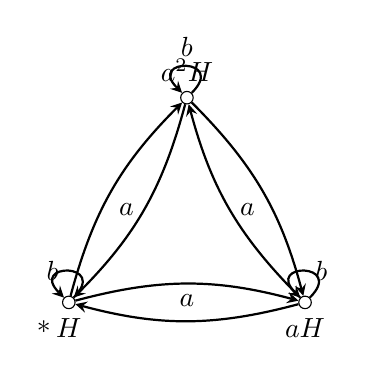
\begin{tikzpicture}[>=stealth,
                    vertex/.style={circle,draw,inner sep=1.6pt,font=\small},
                    edge/.style={thick},
                    loop/.style={edge,->,looseness=8,min distance=18pt}]

  % 三个顶点(余类)
  \node[vertex,label=below:$H$]              (H)   at (0,0) {};
  \node[vertex,label=below:$aH$]             (aH)  at (3,0) {};
  \node[vertex,label=above:$a^{2}H$]         (a2H) at (1.5,2.6) {};

  % a-边:顺时针画成一个三角形(有向边可按需要加/去 arrow)
  \draw[edge,->] (H)   to[bend left=15] node[below] {$a$} (aH);
  \draw[edge,->] (aH)  to[bend left=15] node[right] {$a$} (a2H);
  \draw[edge,->] (a2H) to[bend left=15] node[left]  {$a$} (H);

  % (可选)补上逆向的 a-边,得到双向箭头
  \draw[edge,->] (aH)  to[bend left=15] (H);
  \draw[edge,->] (a2H) to[bend left=15] (aH);
  \draw[edge,->] (H)   to[bend left=15] (a2H);

  % b-边:每个顶点上一条自环
  \draw[loop] (H)   to node[left]  {$b$} (H);
  \draw[loop] (aH)  to node[right] {$b$} (aH);
  \draw[loop] (a2H) to node[above] {$b$} (a2H);

  % (可选)基点
  \node at (H) [below left=3pt] {$\ast$};
\end{tikzpicture}
\end{document}
